%!TEX root = ../main.tex

\chapter{Background biologico}\label{chp:biological-background}

La cellula è l'unità fondamentale della vita. La cellula è una piccola miscela acquosa con componenti chimici, racchiusi in una membrana, e possiede l'eccezionale capacità di replicarsi. Il primo elemento che permette di distinguere le cellule è la presenza di un nucleo. Vengono definite \textsl{procarioti} le cellule senza nucleo — che sono le più diffuse e compongono organismi unicellulari come i batteri e gli archei — mentre sono chiamate \textsl{eucarioti} le cellule che contengono un nucleo — le quali sono in genere più grandi e più complesse e costituiscono forme di vita multicellulari come animali, piante e funghi\,\cite{alberts2015essential}.

All'interno della cellula eucariote (Figura\,\ref{fig:cell}), immersi nel \textsl{citoplasma}, sono presenti diversi \textsl{organuli}, i quali svolgono una particolare funzione ciascuno. I \textsl{mitocondri} sono gli organuli più diffusi.
% 
\begin{figure}[b!]
    \centering
    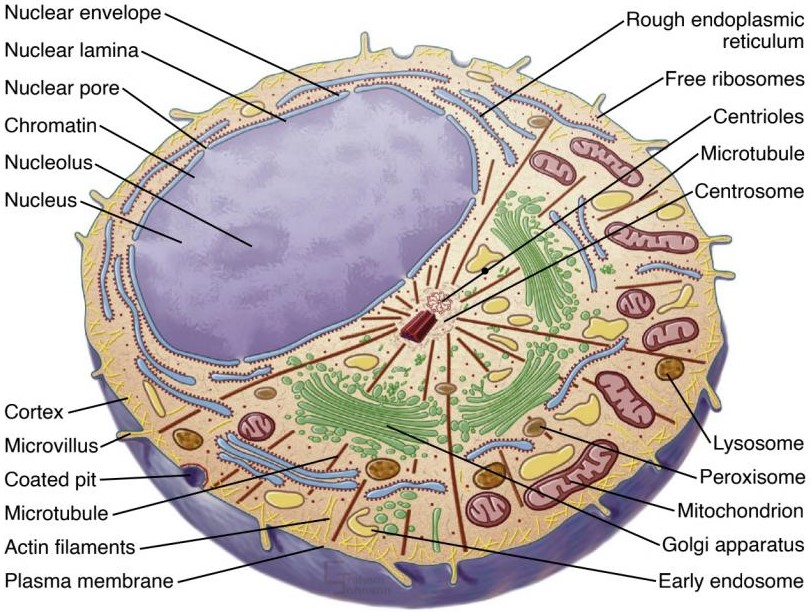
\includegraphics[width=.65\textwidth]{assets/imgs/cell.jpg}
    \caption[Rappresentazione schematica della cellula eucariote.]{Rappresentazione schematica della cellula eucariote; si possono notare i principali organuli tra cui i mitocondri, lisosomi e perossiomi, il reticolo endoplasmatico, e il nucleo\,\cite{pollard2022cell}.}\label{fig:cell}
\end{figure}
% 
Il loro compito è quello di generare energia chimica per la cellula: attraverso il processo di ossidazione di zuccheri e grassi, viene creata una sostanza che viene utilizzata nella maggior parte delle attività cellulari\footnote{Questa sostanza è detta \textsl{adenosintrifosfato} o \acs{ATP} ed ha una struttura simile ad un nucleotide: è infatti composta dall'Adenina, da uno zucchero e da tre gruppi fosfati.}; questo processo è anche chiamato \textsl{respirazione cellulare} perché consumando l'ossigeno viene rilasciata anidride carbonica. Oltre ad essere la fonte energetica primaria della cellula, i mitocondri hanno anche importanti ruoli nella regolazione del metabolismo, del ciclo cellulare, delle risposte antivirali e anche della morte della cellula\,\cite{alberts2015essential, chinnery2003mitochondria, mcbride2006mitochondria}.

Il \textsl{reticolo endoplasmatico} è invece un organulo molto esteso e svolge molteplici funzioni. Tra questi compiti rientrano quelli di traslocazione di proteine e il ripiegamento delle proteine (\textsl{protein folding})\,\cite{alberts2015essential, voeltz2002structural}. I \textsl{lisosomi} si occupano di degradare e riciclare gli scarti cellulari e giocano un ruolo fondamentale per l'omeostasi della cellula\footnote{Con omeostasi cellulare si intende l'insieme di meccanismi necessari per mantenere ad un livello ottimale le funzioni della cellula.}, il suo sviluppo e il suo invecchiamento\,\cite{ballabio2016awesome, yang2021lysosome, dell2000lysosome}. Infine, i \textsl{perossiomi} sono delle piccole vescicole che forniscono un ambiente protetto per gestire molecole tossiche come gli acidi grassi i quali sono smaltiti tramite la $\beta$-ossidazione\,\cite{alberts2015essential, islinger2012peroxisome}.

L'organulo più importante della cellula rimane il \textsl{nucleo}. Racchiuso nell'\textsl{involucro nucleare}, all'interno di questo organulo sono presenti tutte le informazioni genetiche, racchiuse in una lunga molecola di acido desossiribonucleico (comunemente noto come \acs{DNA}), che, una volta impacchettato forma il \textsl{cromosoma}\,\cite{pollard2022cell, alberts2015essential}. La molecola di \acs{DNA} è una struttura a doppia elica formata da \textsl{nucleotidi}. Osservando la Figura\,\ref{fig:dna}, i nucleotidi sono composti a loro volta da tre elementi fondamentali: una \textsl{base azotata}, uno \textsl{zucchero} e un \textsl{gruppo fosfato}\footnote{I gruppi fosfati hanno una carica negativa e forniscono alla molecola le proprietà di un acido.}.
% 
\begin{figure}[b!]
    \centering
    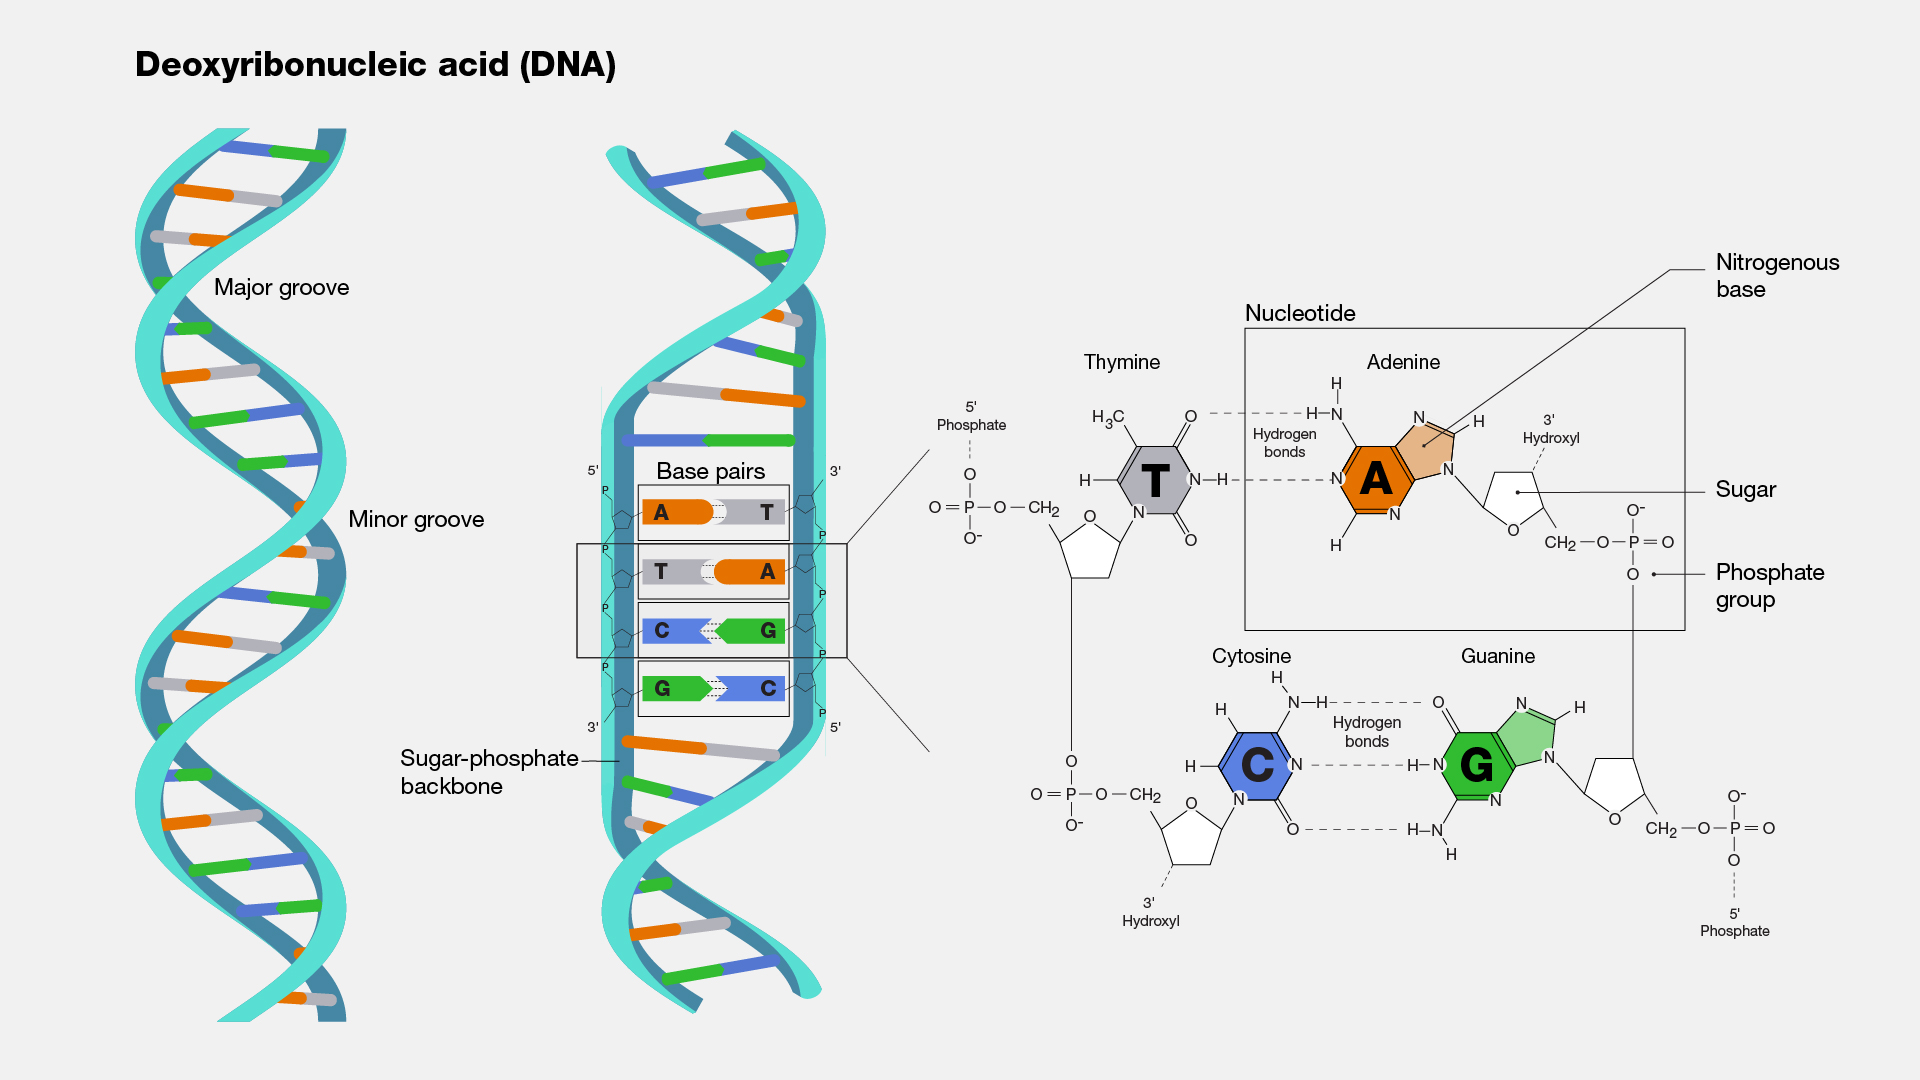
\includegraphics[width=\textwidth]{assets/imgs/dna.jpg}
    \caption[Rappresentazione schematica del \acs{DNA}.]{Rappresentazione schematica del \acs{DNA} in cui si possono osservare le coppie di basi azotate, legate tra loro attraverso gli zuccheri e i gruppi fosfati\,\cite{nhgri_dna_image}.}\label{fig:dna}
\end{figure}
% 
Le basi azotate sono quattro — Adenina (A), Citosina (C), Guanina (G) e Timina (T) — e si uniscono tra loro mediante dei legami ad idrogeno e secondo un preciso criterio: l'Adenina si lega solamente con la Timina (formando il legame \textit{AT}) mentre la Citosina si unisce solo con la Guanina (creando la coppia \textit{CG})\,\cite{fonseca2000hydrogen, sahu2011identification}. Si osserva infine che il nucleotide di una coppia e quello successivo si legano mediante zucchero e gruppo fosfato sempre allo stesso modo: il gruppo fosfato di un nucleotide si lega sempre allo zucchero dell'altro. Di conseguenza, preso un filamento della doppia elica, le due estremità non sono uguali in quanto una termina con un gruppo fosfato (terminazione $5^\prime$) e l'altra con uno zucchero (terminazione $3^\prime$).

Attraverso una serie di ripiegamenti, una molecola di \acs{DNA} lunga circa due metri riesce a raggomitolarsi in un cromosoma di grandezza inferiore a 2 micron (Figura\,\ref{fig:dna-packaging}). Il processo di \textit{\acs{DNA}-packaging} inizia avvolgendo la doppia elica di \acs{DNA} attorno a delle proteine dette \textsl{istoni} e formando dei \textsl{nucleosomi}. In secondo luogo i nucleosomi si ammassano vicini tra loro formando una fibra, chiamata \textsl{cromatina} che, a sua volta si impacchetta su se stessa creando il cromosoma\,\cite{jansen2011nucleosome, zheng2010packaging}.

\begin{figure}[b!]
    \centering
    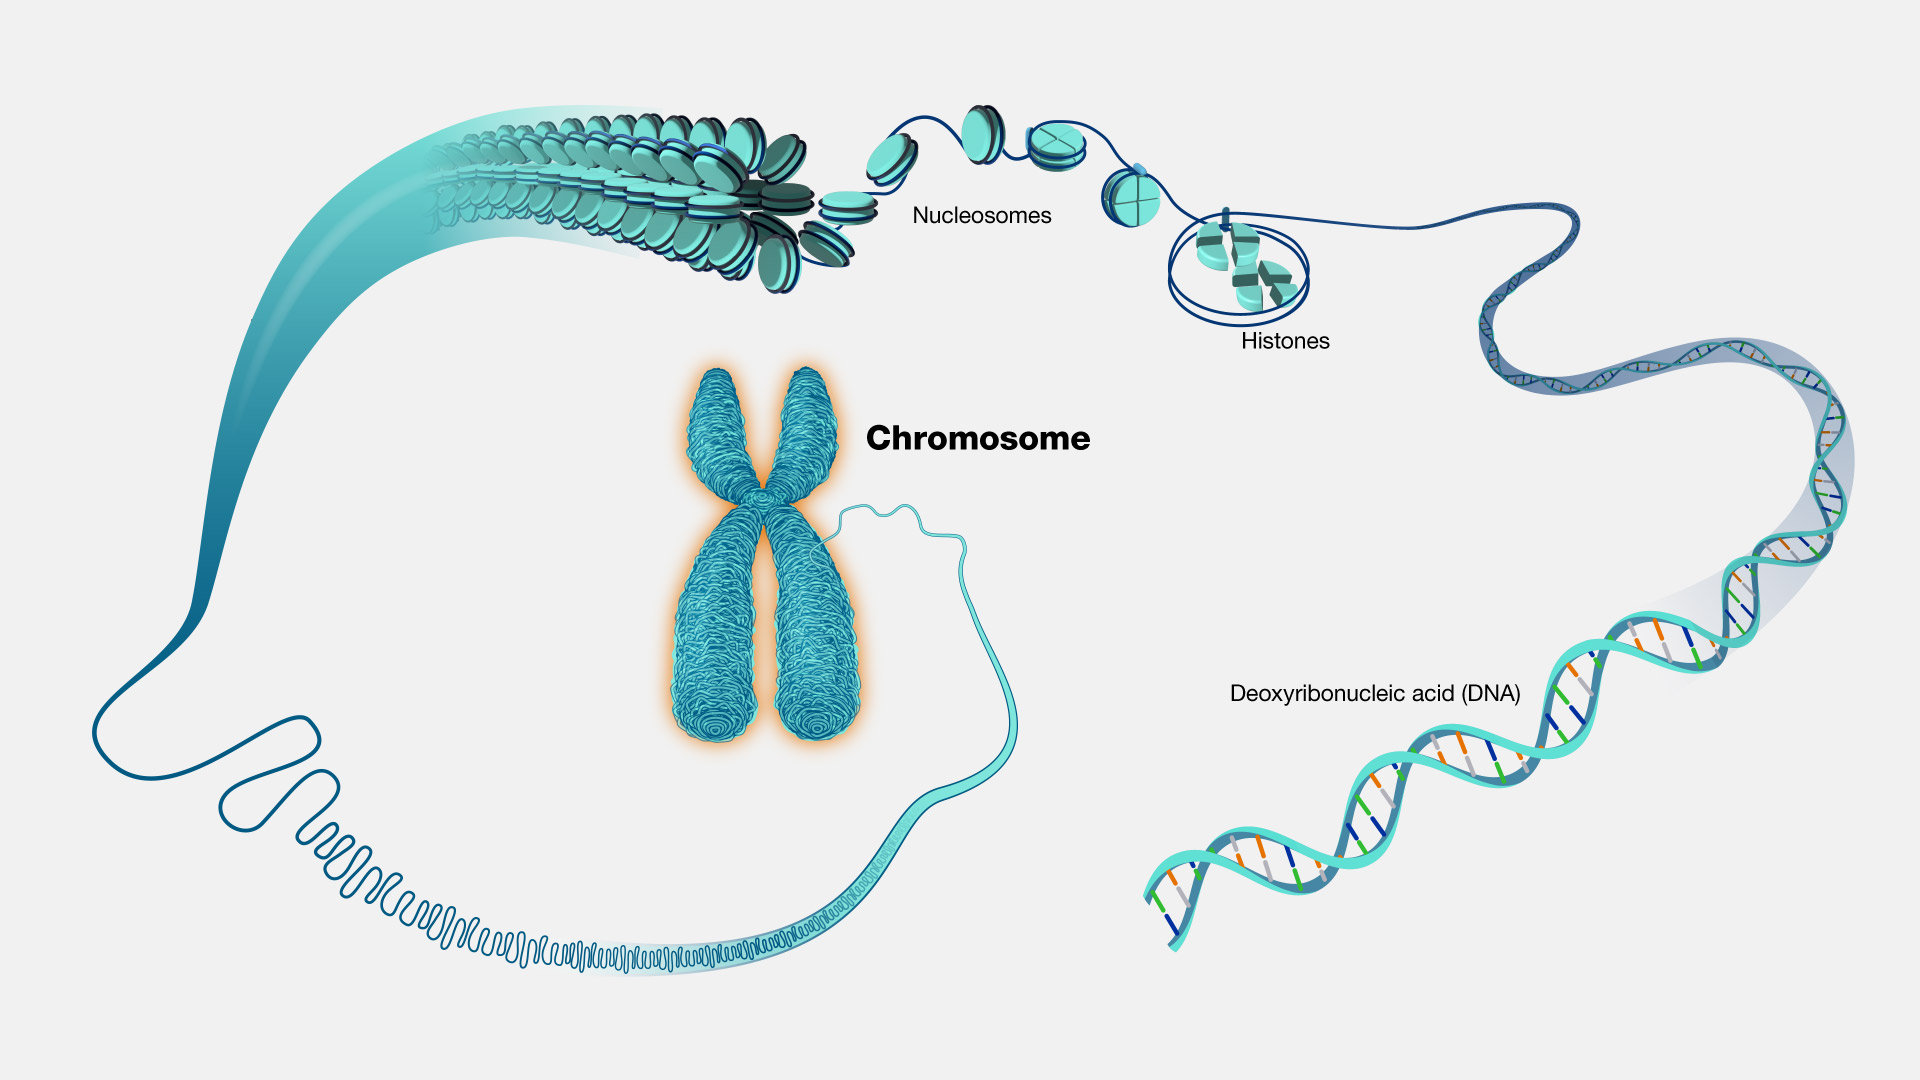
\includegraphics[width=\textwidth]{assets/imgs/dna-packaging.jpg}
    \caption[Il processo di impacchettamento del \acs{DNA}.]{Il processo di impacchettamento del \acs{DNA} che permette di compattare la struttura a doppia eilca nel cromosoma\,\cite{nhgri_chromosome_image}.}\label{fig:dna-packaging}
\end{figure}

\section{Dogma centrale}

La rilevanza del \acs{DNA} è data delle informazioni essenziali che questa molecola contiene. Tali informazioni risiedono nei geni, che sono delle sequenze genomiche che codificano uno o più prodotti biologici operativi\,\cite{gerstein2007gene}. L'\textsl{espressione genica} è il processo che permette di utilizzare i dati contenuti nel gene per la creazione di macromolecole, come le proteine. Per esempio, le cellule della pelle a contatto con luce solare intensa possono esprimere geni che regolano la pigmentazione della pelle\,\cite{white2009gene}. L'espressione genica è divisa in due fasi principali: la \textsl{trascrizione} — che si occupa di produrre delle molecole di \acs{RNA} che rispecchino il gene da esprimere — e la \textsl{traduzione} — la quale traduce le informazioni dell'\acs{RNA} sintetizzando la proteina.

Nella prima fase dell'espressione genica, è necessario trascrivere il \acs{DNA} in una molecola molto simile ovvero l'\acs{RNA} — chiamato anche acido ribonucleico. Questa molecola differisce dall'acido desossiribonucleico per una base azotata — anziché la Timina è presente l'Uracile (U) — e per lo zucchero — da desossiribosio a ribosio\,\cite{alberts2002dna}. La trascrizione del \acs{DNA} in \acs{RNA} inizia quando delle proteine, chiamate \textsl{fattori di trascrizione} (\acs{TF}), attratte dagli \textit{enhancer} del \acs{DNA}, riconoscono la regione che delimita l'inizio della molecola del gene da esprimere, detta \textit{promoter}. Dopo aver riconosciuto l'inizio della sequenza, queste proteine permettono ad un enzima chiamato \textsl{\acs{RNA} polimerasi} di attaccarsi ed aprire la doppia elica del \acs{DNA}\,\cite{cramer2019organization}. Una volta aperta la doppia elica, inizia la vera e propria trascrizione in \acs{RNA}:\@ il filamento del \acs{DNA} viene preso come modello per la creazione dell'\acs{RNA};\@ in particolare il nucleotide dell'\acs{RNA} sarà il complementare rispetto a quello del \acs{DNA} (di conseguenza $A\rightarrow U$, $C\rightarrow G$, $G\rightarrow C$ e $T\rightarrow A$). Così facendo l'acido ribonucleico viene creato un nucleotide alla volta, analizzando quello del \acs{DNA}\,\cite{alberts2002dna}. La trascrizione termina nel momento in cui gli enzimi e le proteine incontrano la regione terminatrice del gene che determina la separazione dal filamento e la terminazione dell'\acs{RNA} \textsl{messaggero} (\acs{mRNA}) che contiene le informazioni presenti nel gene da esprimere. L'intero processo di trascrizione è illustrato nella Figura\,\ref{fig:dna-transcription}.

\begin{figure}[b!]
    \centering
    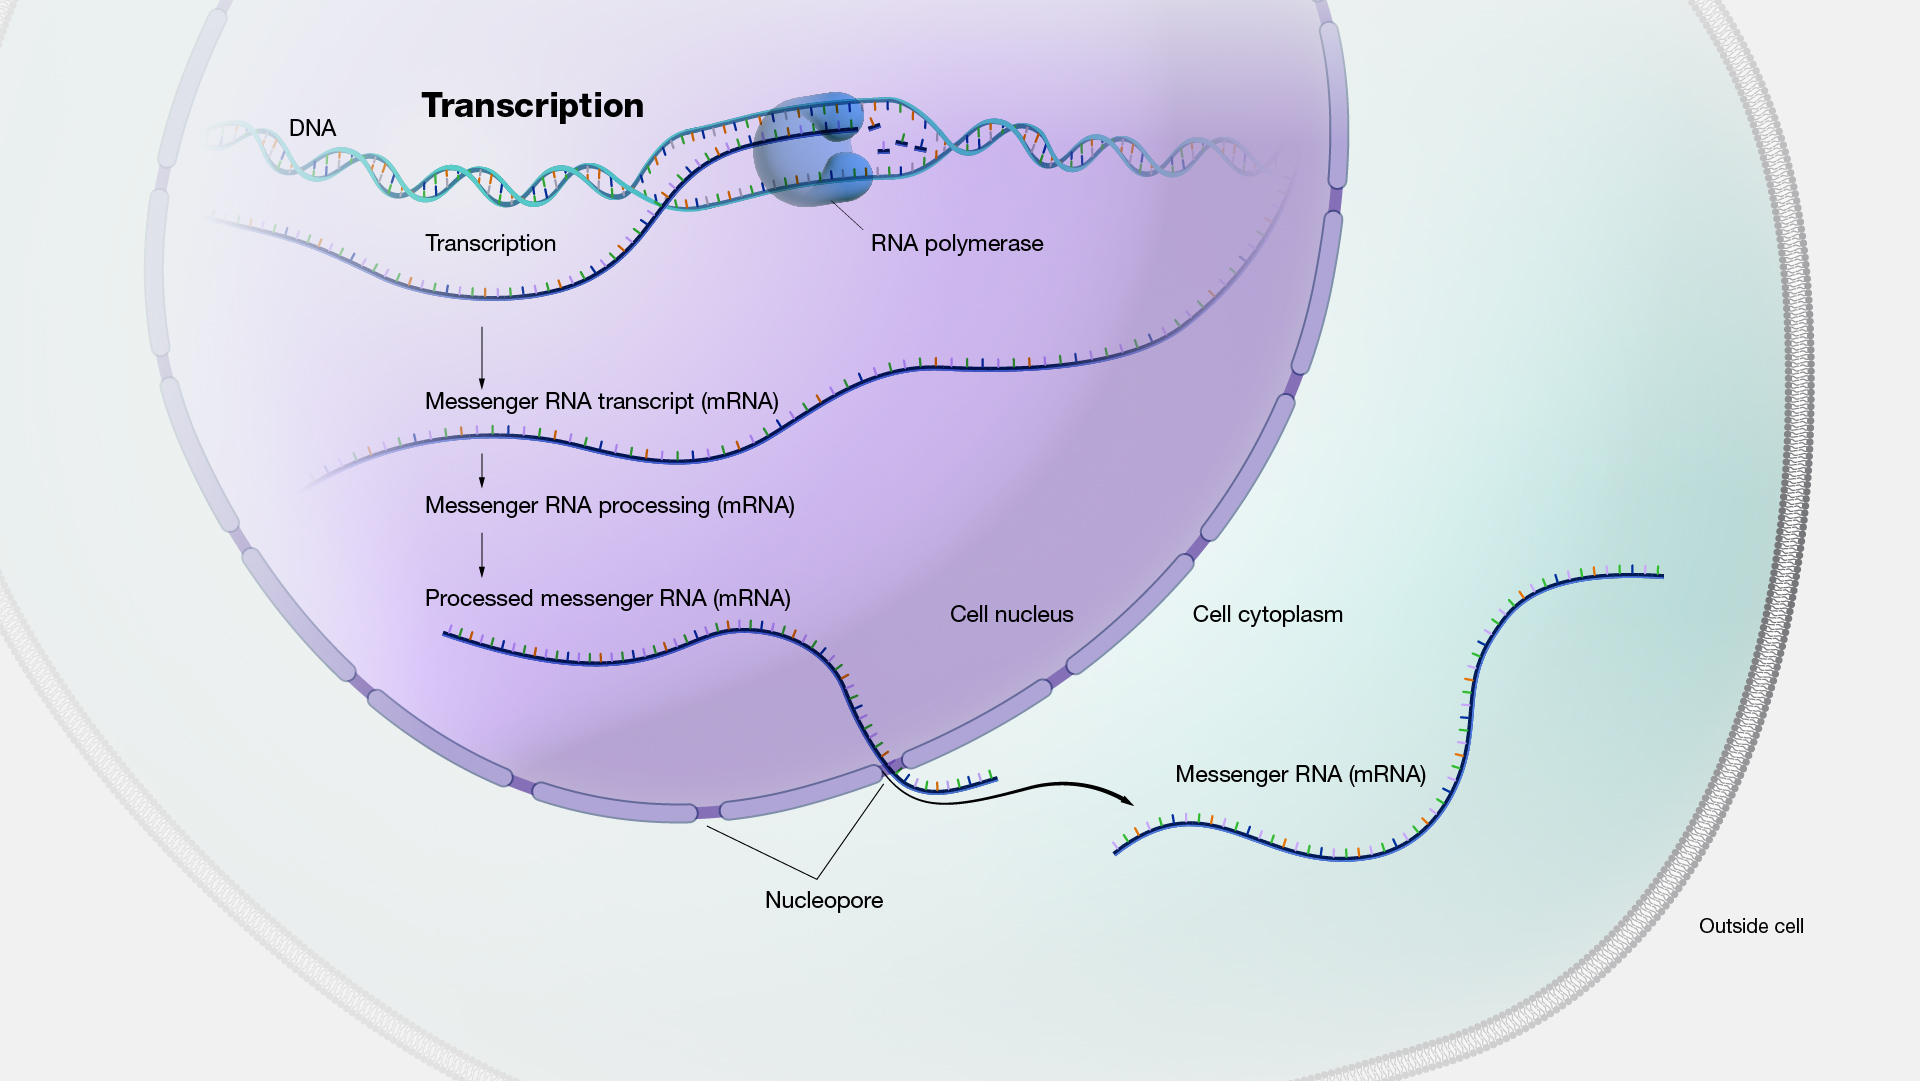
\includegraphics[width=\textwidth]{assets/imgs/dna-transcription.jpg}
    \caption[Il processo di trascrizione del \acs{DNA} in \acs{RNA}.]{Il processo di trascrizione del \acs{DNA} del gene in \acs{RNA} mediante la \acs{RNA} polimerasi\,\cite{nhgri_transcription_image}.}\label{fig:dna-transcription}
\end{figure}

Prima di uscire dal nucleo l'\acs{RNA} messaggero subisce una serie di elaborazioni necessarie per rendere le informazioni immagazzinare sicure: diverse sono le malattie che emergono per mutazioni presenti nell'\acs{mRNA} tra cui la distrofia miotonica\footnote{Le distrofie miotoniche sono patologie che colpiscono principalmente l'apparato muscolo-scheletrico.}\,\cite{philips2000rna}. La prima elaborazione viene chiamata $5^\prime$-\textit{end capping} e si occupa di aggiungere alla terminazione $5^\prime$ dell'\acs{mRNA} una Guanina attraverso un collegamento inusuale che garantisce maggiore stabilità alla molecola. In secondo luogo avviene lo \textit{splicing} che si occupa di rimuovere le zone non codificanti — dette \textsl{introni}— dal gene trascritto mantenendo solo quelle che verranno utilizzate per essere sintetizzate in proteine — gli \textsl{esoni} — e quindi facilitando il processo di traduzione. Infine con il $3^\prime$-\textit{end processing} viene aggiunta alla terminazione $3^\prime$ dell'\acs{mRNA} una coda di Adenine — datta anche \textit{poly}A \textit{tail} — che, in maniera molto simile al $5^\prime$-\textit{end capping} garantisce una stabilità del filamento di acido ribonucleico\,\cite{hocine2010rna, livingstone2010mechanisms}.

Dopo essere uscito dal nucleo attraverso i \textsl{pori}, l'\acs{RNA} messaggero raggiunge il citoplasma ed è pronto per iniziare la seconda fase dell'espressione genica, la traduzione. La traduzione non è altro che la traduzione dell'\acs{mRNA} in un \textsl{polipeptide}, ovvero una sequenza di aminoacidi che compongono la proteina. Gli aminoacidi sono più di 20, di conseguenza anziché codificare un solo nucleotide dell'\acs{RNA} messaggero, vengono codificati tre nucleotidi alla volta: questa tripletta viene chiamata \textsl{codone}. Durante la fase della traduzione, giocano un ruolo fondamentale i \textsl{ribosomi} i quali sono degli organuli nei quali avviene la traduzione. I ribosomi sono composti da due sotto unità, ciascuna delle quali ha tre siti per l'\acs{RNA} di \textsl{trasporto} (\textsl{tRNA}). Delle due sotto unità del ribosoma, quella dimensionalmente minore si lega all'\acs{mRNA} e agli \textsl{anticodoni} (sequenze specifiche di tre basi nel tRNA) e controlla che la traduzione avvenga con successo. La sotto unità più voluminosa invece si prende carico di catalizzare il legame peptidico tra l'aminoacido trasportato dal tRNA e la catena di aminoacidi in crescita\,\cite{ramakrishnan2002ribosome, lemonniermarathon, livingstone2010mechanisms}. In questo modo i ribosomi, analizzando codone dopo codone riescono a creare la catena polipeptidica mediante l'\acs{RNA} di trasporto, come mostrato nella Figura\,\ref{fig:mrna-translation}.

\begin{figure}[b!]
    \centering
    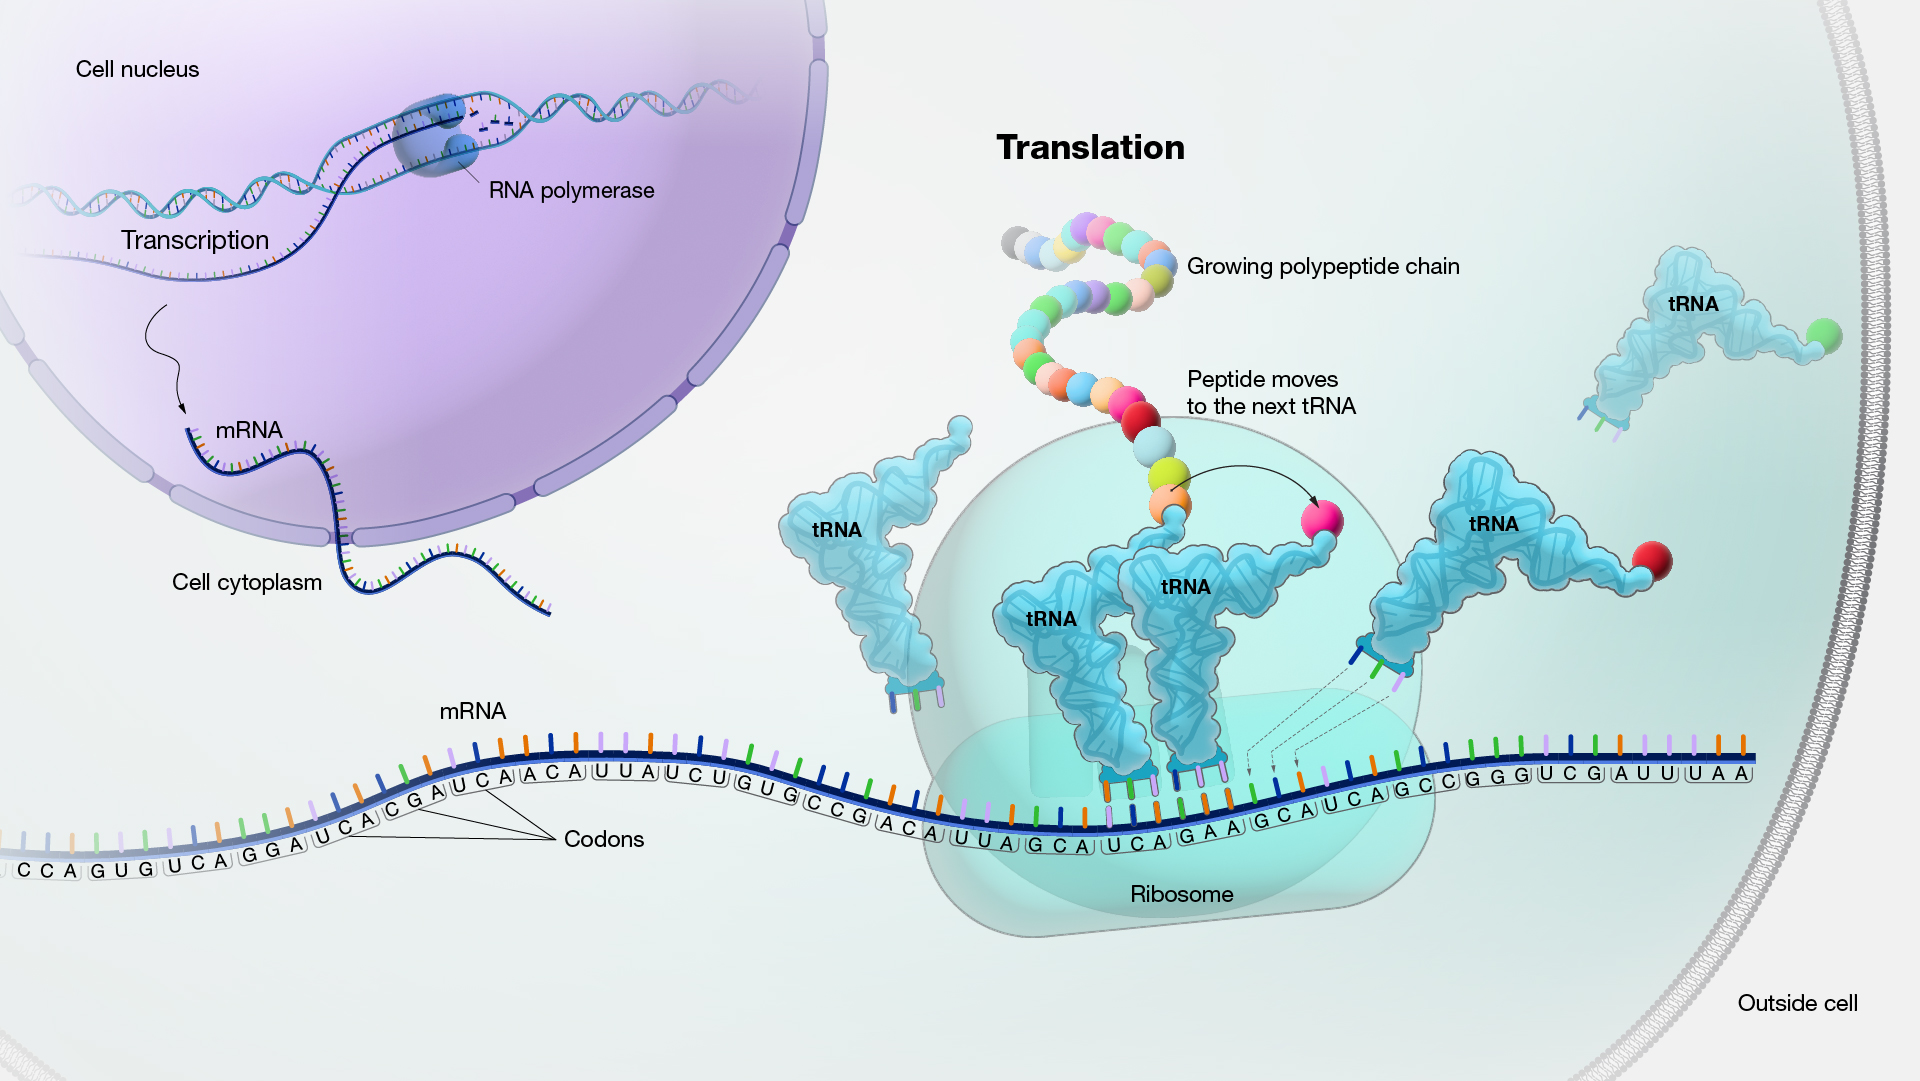
\includegraphics[width=\textwidth]{assets/imgs/mrna-translation.jpg}
    \caption[Il processo di traduzione da \acs{mRNA} a polipeptide.]{Il processo di traduzione da \acs{RNA} messaggero a polipeptide attraverso il tRNA e i ribosomi\,\cite{nhgri_translation_image}.}\label{fig:mrna-translation}
\end{figure}

Una volta creata la sequenza polipeptidica, inizia il processo di ripiegamento della proteina. In maniera molto simile a quanto visto per l'impacchettamento del \acs{DNA} nel cromosoma, la sequenza di polipeptidi inizialmente si arrotola creando delle bobine che sono comunemente chiamate $\alpha$\textit{-helix}. Queste ultime poi si ripiegano nuovamente arrivando alla struttura terziaria della proteina, ovvero la proteina tridimensionale effettiva\,\cite{schulz2013principles}. Una volta creata la proteina il gene è stato espresso definitivamente. Questo passaggio di informazioni dal \acs{DNA} alla creazione della proteina è gergo definito come il \textsl{dogma della biologia molecolare}.

Come accennato all'inizio del capitolo, la cellula possiede la notevole capacità di replicarsi. In genere una cellula si duplica durante la crescita e lo sviluppo dell'organismo, quando deve essere rimpiazzata o rigenerata oppure nella riproduzione asessuata di alcuni micro organismi\,\cite{bavle2014mitosis}. Il processo replicazione cellulare, chiamato \textsl{mitosi}, è preceduto dall'\textsl{interfase}, processo fondamentale in cui la cellula cresce di dimensioni e il \acs{DNA} nei cromosomi si duplica, favorendo la replicazione cellulare. La mitosi può essere suddivisa in quattro fasi principali\,\cite{walczak2010mechanisms, bavle2014mitosis, li2020theoretical, sullivan2007finishing} le quali sono riassunte anche nella Figura\,\ref{fig:mitosis}:
\begin{enumerate}
    \item Nella \textsl{profase} i cromosomi duplicati si condensano nel nucleo ed iniziano ad avvicinarsi dei microtuboli al nucleo, chiamati \textsl{centrosomi}; allo stesso tempo la membrana nucleare inizia a svanire;
    \item Dopo che i microtuboli si sono attaccati ai cromosomi (fase intermedia detta \textsl{prometafase}) si giunge alla \textsl{metafase}, situazione in cui tutti i cromosomi sono allineati lungo la linea equatoriale della cellula;
    \item Durante l'\textsl{anafase}, ciascuna coppia di cromosomi si divide e raggiunge i poli della cellula;
    \item La fase finale della mitosi è la \textsl{telofase} nella quale le due cellule si dividono; le membrane nucleari delle due cellule si riformano attorno ai cromosomi divisi.
\end{enumerate}

\begin{figure}[b!]
    \centering
    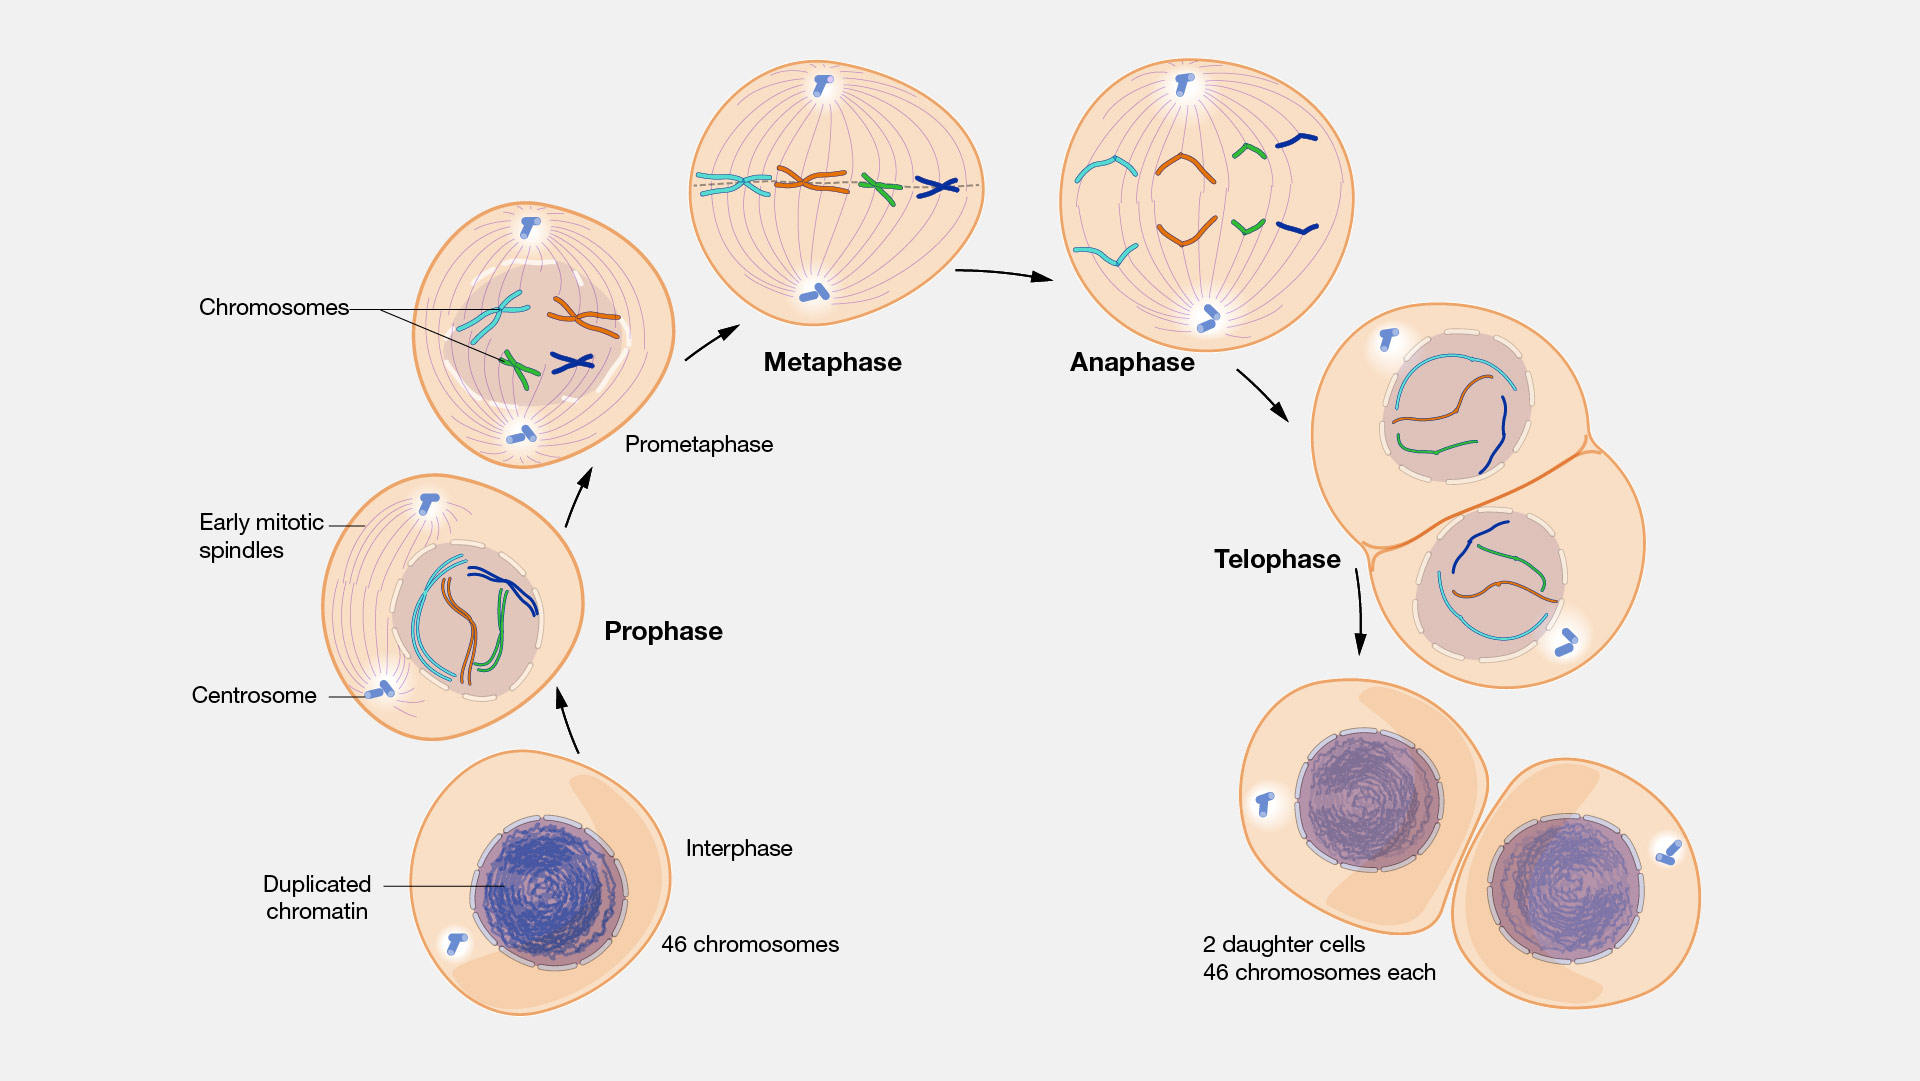
\includegraphics[width=\textwidth]{assets/imgs/mitosis.jpg}
    \caption[La mitosi cellulare.]{Rappresentazione delle quattro fasi che comprendono la mitosi cellulare\,\cite{nhgri_mitosis_image}.}\label{fig:mitosis}
\end{figure}

Affinché la mitosi abbia successo, è prima necessario duplicare il \acs{DNA} all'interno della cellula. Il processo di replicazione di \acs{DNA} che precede la mitosi è anche definito come \textsl{fase di sintesi} — \textit{S-phase}. La duplicazione del \acs{DNA} inizia con l'identificazione dell'\textsl{origine della replicazione}, ovvero una sequenza del \acs{DNA} che specifica da quale punto della sequenza il \acs{DNA} deve essere replicato (ci sono più di cento mila siti che segnalano un punto di orine nel \acs{DNA} di una cellula). Una \textsl{proteina iniziatrice} è legata al punto di origine promuovendo l'attaccamento al \acs{DNA} del \textsl{replisoma} che è composto da un enzima chiamato \textsl{elicasi} che si occupa di dividere i due filamenti di \acs{DNA} procedendo nella direzione $5^\prime \to 3^\prime$.\@ A questo punto il \textsl{\acs{RNA} prime} inizia la sintesi del \acs{DNA} favorendo l'attaccamento della \textsl{\acs{DNA} polimerasi} entrambi i filamenti per duplicare il \acs{DNA}.\@ Essendo che il genoma è complementare, un filamento avrà un verso $5^\prime \to 3^\prime$ (\textit{leading strand}) mentre l'altro filamento avrà verso opposto, $3^\prime \to 5^\prime$ (\textit{lagging strand}). Di conseguenza, nel filamento concorde al replisoma, la polimerasi non incontrerà problemi nella duplicazione, invece nel filamento $3^\prime \to 5^\prime$ il \acs{DNA} dovrà essere duplicato a segmenti, detti \textsl{frammenti di Okazaki} che verranno collegati tramite la \textsl{\acs{DNA} ligasi}\,\cite{laskey1989s, bell2002dna, dutta1997initiation, 2017727}. La Figura\,\ref{fig:dna-replication} racchiude quanto descritto sulla fase di sintesi.

\begin{figure}[b!]
    \centering
    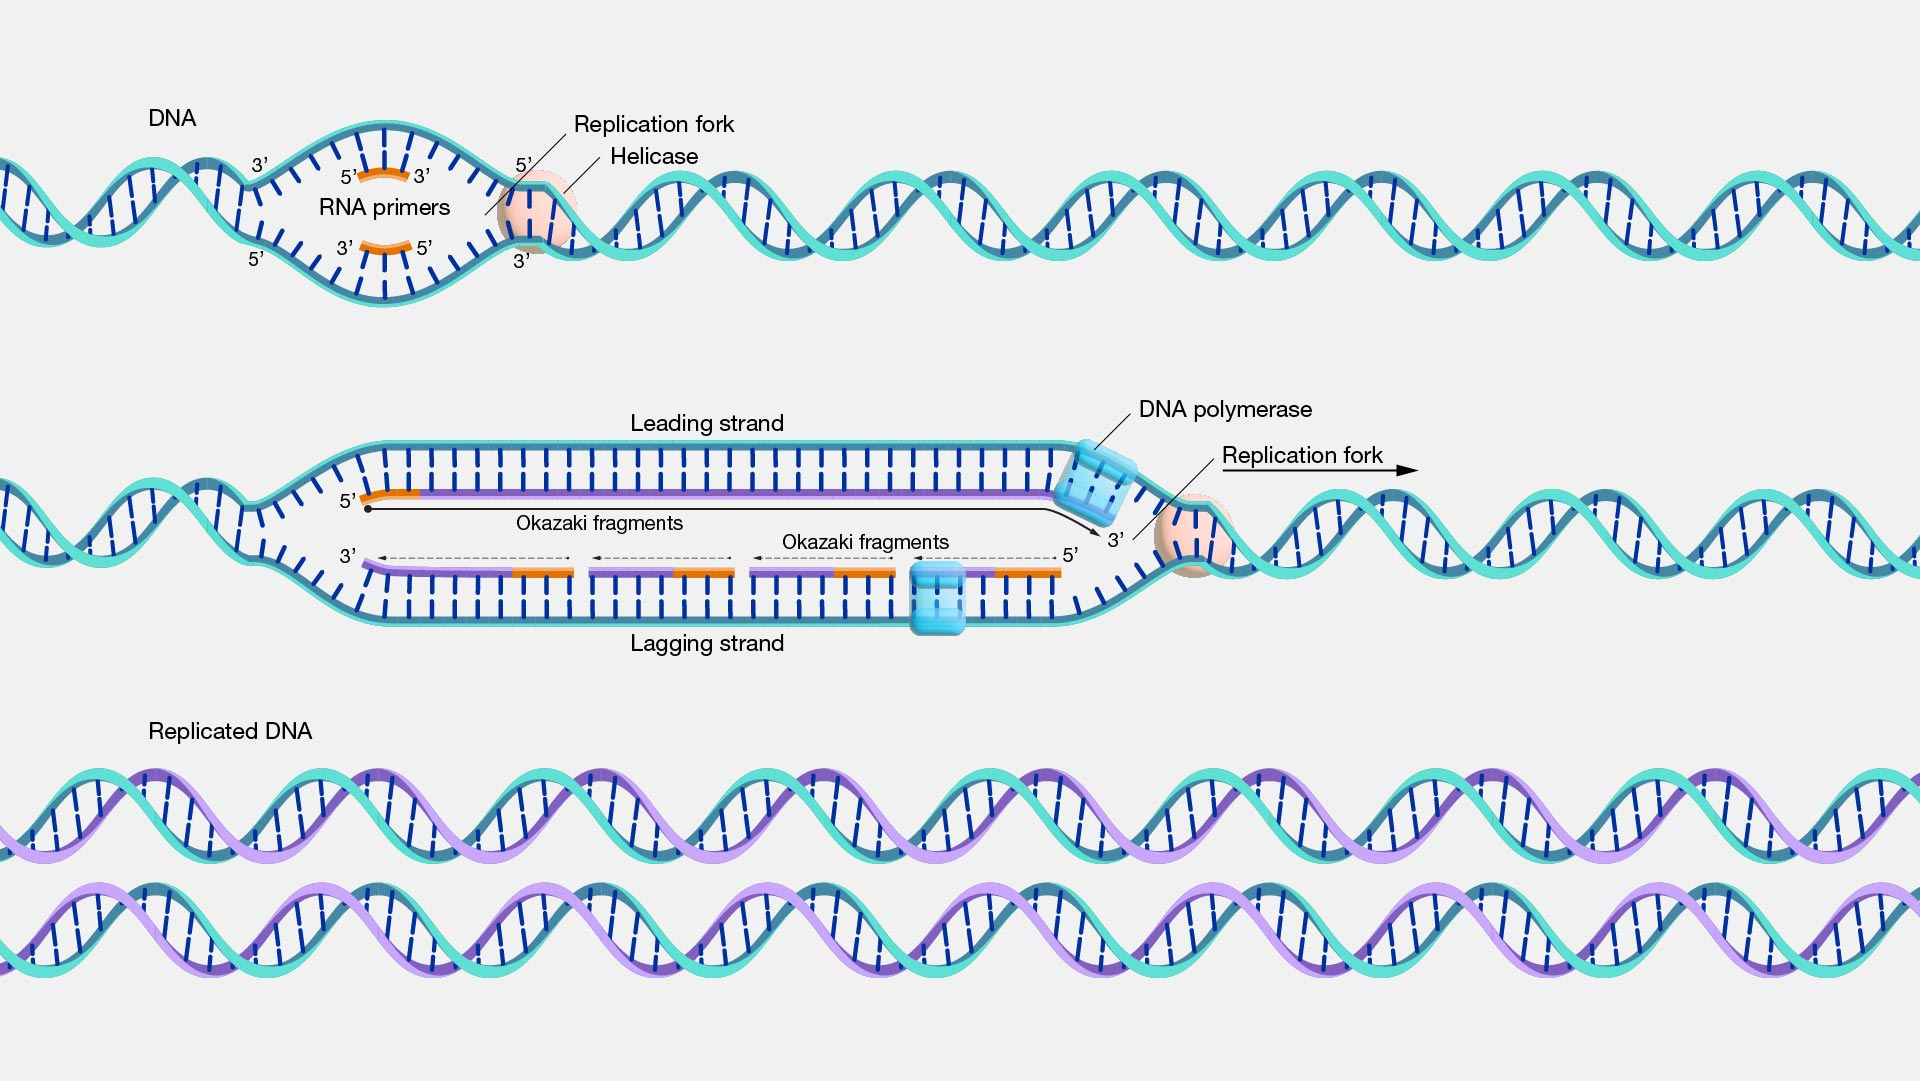
\includegraphics[width=\textwidth]{assets/imgs/dna-replication.jpg}
    \caption[Il processo di replicazione del \acs{DNA}.]{Il processo di replicazione del \acs{DNA} durante la fase di sintesi\,\cite{nhgri_dna_replication_image}.}\label{fig:dna-replication}
\end{figure}

\section{Varianti non codificanti}

Come descritto fino ad ora, il ruolo del \acs{DNA} è fondamentale in quanto trasmesso da cellula a cellula durante la replicazione per poi essere utilizzato nell'espressione genica creando le proteine. Alle regioni del \acs{DNA} che prendono parte all'espressione genica, si contrappongono le regioni che non vengono codificate, come gli enhancers ed i promoters, ma anche gli introni di un gene. Le regioni non codificanti del \acs{DNA} rappresentano tra il 98\% e il 99\% dell'intera molecola: si pensava che queste zone non avessero una funzione effettiva, tanto che vennero definite \textit{junk \acs{DNA}}, ovvero \acs{DNA} spazzatura. Contrariamente a quanto si supponeva, mutazione in queste zone può causare diversi disturbi genetici in quanto l'organizzazione della cromatina, il processo di replicazione del \acs{DNA} e l'espressione genica possono essere compromessi. Nel comprendere l'associazione tra varianti genomiche e disturbi da esse causati, il \textit{Genome-Wide Association Study} (\acs{GWAS}) ha svolto un ruolo rilevante, analizzando genomi di numerosi soggetti e correlando la presenza di una mutazione e un disturbo. Tra le varianti identificata dal \acs{GWAS}, diverse sono mutazioni non codificanti\,\cite{visscher2012five, zhang2015non, ludwig2002functional}.

Alcune varianti non codificanti possono alterare lo splicing di un gene trascritto. Come accennato precedentemente, lo splicing è il processo che permette la rimozione delle zone non codificanti del gene (gli introni) prima che questo sia tradotto in una proteine. Lo splicing fa parte dei processi che l'\acs{mRNA} subisce prima di lasciare il nucleo ed iniziare la traduzione. All'interno degli introni sono presenti diverse sequenze che sottolineano l'inizio di un esone, tra cui il \textit{donor}, l'\textit{acceptor}, i \textit{branch points} e i \textsl{tratti polipirimidinici}. Le variazioni in queste regioni possono condurre alla non codifica di un esone o alla conservazione di un introne: più del 15\% dei disturbi ereditari sono dovuti proprio a questi inconvenienti. Oltre agli introni, anche altre regioni non tradotte (\acs{UTR}) dell'\acs{mRNA} possono condurre ugualmente a disturbi ereditari. Queste regioni sono fondamentali per gestire il processo seguente alla trascrizione: si occupano infatti di rendere il filamento di \acs{mRNA} più stabile e robusto e rendono la sua localizzazione più semplice per poter iniziare il processo di traduzione\,\cite{khurana2016role, french2020role}. 

Le mutazioni non codificanti, oltre a verificarsi nell'\acs{RNA} messaggero, possono anche occorrere nelle regioni non codifcianti del \acs{DNA} (\acs{ncDNA}), come i promoters i quali attirano i fattori di trascrizione (\acs{TF}). Queste proteine sono responsabili di agganciare alla molecola di \acs{DNA} la \acs{RNA} polimerasi, che si occupa di sciogliere la doppia elica ed inizia la trascrizione del gene. La variazione di queste importanti regioni rende la trascrizione del gene incorretta, conducendo ad un'erronea traduzione in proteina. Le variazione dei promoter sono causa di malattie mendeliane e di alcuni tipi di tumori. Per lo stesso motivo, anche le mutazioni in altre sequenze \textsl{cis-regolatorie} del \acs{DNA} — come enhancers e \textit{silencers}\footnote{A differenza degli enhancer, che stimolano una particolare trascrizione genica, lo scopo dei silencers è quello di ridurre o inibire la trascrizione di un particolare gene} — conducono a malattie ereditarie. Tra questi disturbi, oltre a quelli citati precedentemente si aggiungono l'aritmia cardiaca, la sindrome della gamba senza riposo\footnote{Questa sindrome neurologica suscita al soggetto una insopportabile necessitàdi muovere gli arti inferiori.} e agenesia pancreatica\footnote{Questo disturbo determina l'assenza di massa pancreatica sin dalla nascita.}\,\cite{zhang2015non, french2020role, pagni2022non, khurana2016role}.

In aggiunta alle variazioni di enhancers e promoters del \acs{DNA} non codificante, le mutazioni possono causare anche l'espansione dei \textit{tandem repeats}, sia negli esoni, che in regioni non codificanti del \acs{DNA}. I tandem repeats sono delle lunghe ripetizioni di ridotte sequenze di \acs{DNA}. Le conseguenze delle viariazioni dei repeat codificanti sono ben note (tra cui il morbo di Huntington), contrariamente all'effetto dell'espansione dei repeat non codificanti. A queste mutazioni si associano disturbi nella fase di trascrizione del \acs{DNA} e l'intrappolamento delle proteine coinvolte durante lo splicing\,\cite{french2020role}.

Le mutazioni del \acs{ncDNA}, possono anche introdurre dei cambiamenti strutturali della cromatina, fibra che costituisce i cromosomi. In particolare, la cromatina, mentre si impacchetta per formare il cromosoma (Figura\,\ref{fig:dna-packaging}), forma delle particolari regioni, dette \acs{TAD} (\textit{Topologically Associating Domains}), le quali contengono gruppi di geni che interagiscono frequentemente tra loro. Ne consegue che anche una piccola variazione strutturale può condurre ad una espressione genica imperfetta, causata da una socorretta interazione tra enhancers e promoters. Si è osservato che la variazione strutturale delle \acs{TAD}, oltre a causare disturbi mendeliani, può portare a diverse malattie neurologiche\,\cite{french2020role, kaiser2017tads}. Oltre alle \acs{TAD}, anche altre regioni della cromatina hanno un ruolo importante durante la trascrizione, come le regioni ipersensibili alla \textsl{DNasi I}\footnote{È un enzima che scinde il \acs{DNA} in frammenti più piccoli. Spesso è utilizzato per identificare regioni di cromatina che sono più accessibili alla trascrizione.} (dette \acs{DHS}), i siti di legame dei fattori di trascrizione (\acs{TF} \textit{binding sites}) e le modifiche istoniche. Queste regioni fanno parte, più in generale delle regioni aperte di cromatina (\acs{OCR}) le quali mutazioni possono portare ad una espressione genica inesatta e, conseguentemente, condurre a disturbi genetici\,\cite{zhou2015predicting, ma2023deepsata}.

Contrariamente alle mutazioni nel \acs{DNA} codificante, gli effetti delle variazioni nel \acs{ncDNA} sono tuttora poco comprese. Questo è dovuto alla difficoltà di determinare se una variante non codificante influenzi effetto sul \textsl{fenotipo} — ovvero l'insieme delle caratterstiche strutturali e funzionali di un individuo. Diversi sono i tool bioinformatici che sono stati sviluppati per riconoscere se una mutazione non codificante abbia un effetto funzionale, ma, poiché tali funzioni dipendono anche dal contesto specifico della sequenza le previsione possono rivelarsi imprecise, fornendo quindi informazioni non del tutto chiare sull'effetto fenotipico della mutazione\,\cite{schipper2022demystifying, pena2024decoding}. 
